\begin{frame}{5.1. Resultados obtenidos: precisión ($+$)}

% \textbf{Precisión (clase positiva).} \underline{BoW, TF-IDF}
% \begin{itemize}
%     \item \textbf{{P-S}\textsubscript{One}.} \underline{BoW + SGD}; BoW, TF-IDF; {DistilBERT}\textsubscript{C \& C, ML}; {BERT}\textsubscript{C \& C/U, ML \& L}; {DeBERTa}\textsubscript{B \& L}; {RoBERTa}\textsubscript{L}\footnote{Los subíndices utilizados para cada modelo $M$ indican respectivamente $M_{\text{B}}$: BASE; $M_{\text{L}}$: LARGE; $M_{C}$: CASED; $M_{\text{U}}$: UNCASED; $M_{\text{ML}}$: MULTILINGUAL.}
%     \item \textbf{{P-S}\textsubscript{All}.} \underline{BoW + NB};  BoW, TF-IDF; {DistilBERT}\textsubscript{B, C, ML}; {DeBERTa}\textsubscript{B}; {M}\textsubscript{L}
%     \item \textbf{News.} \underline{TF-IDF + SGD};  BoW, TF-IDF; $\downarrow$ \textit{transformers} (-0.5 aprox.)
% \end{itemize}

% \end{frame}

% \begin{frame}{Resultados: precisión, \textit{specificity}, \textit{F1} (negativa)}

% \textbf{Precisión (clase negativa).} \underline{BoW, TF-IDF} $>$ {{M}\textsubscript{L}} $\approx$ {{M}\textsubscript{B}}

% \begin{itemize}
%     \item \textbf{{P-S}\textsubscript{One}.} {BoW, TF-IDF} $\approx$ {{M}\textsubscript{B}} $\approx$ {{M}\textsubscript{L}}
%     \item \textbf{{P-S}\textsubscript{All}.} {BoW} $>$ {TF-IDF}, {DistilBERT}, {DeBERTa}\textsubscript{B}, {{M}\textsubscript{L}} $>$ {{M}\textsubscript{B}}
%     \item \textbf{News.} {BoW, TF-IDF} $\gg$ {{M}\textsubscript{B \& L}}
% \end{itemize}

% \vspace{2ex}

% \textbf{\textit{Specificity} (clase negativa).} \underline{{M}\textsubscript{L}} $>$ {BoW, TF-IDF}  $\gg$ {M}\textsubscript{B}
% \begin{itemize}
%     \item \textbf{{P-S}\textsubscript{One}.}
%     \item \textbf{{P-S}\textsubscript{All}.}
%     \item \textbf{News.} {{M}\textsubscript{L}, BoW, TF-IDF} $\gg$ {M}\textsubscript{B}
% \end{itemize}


% \textbf{\textit{F1-Score} (clase negativa).} \underline{BoW, TF-IDF} $\approx$ {M}\textsubscript{L} $>$ {M}\textsubscript{B}
% \begin{itemize}
%     \item \textbf{{P-S}\textsubscript{One}.}
%     \item \textbf{{P-S}\textsubscript{All}.}
%     \item \textbf{News.} {BoW, TF-IDF} $>$ {M}\textsubscript{L} $>$ {M}\textsubscript{B}
% \end{itemize}

Métricas utilizadas: precisión (+, $-$); \textit{specificity} ($-$); \textit{F1-score} ($-$).

\vspace{2ex}

\begin{itemize}
    % \item Precisión (+): 
    \item Mejores modelos:
    \begin{itemize}
        \item {P-S}\textsubscript{One}: BoW + SGD
        \item {P-S}\textsubscript{All}: BoW + NB
        \item News: TF-IDF + SGD
    \end{itemize}
    \item BoW $>$ TF-IDF $>$ LARGE $>$ BASE
    \item CASED, ML $>$ UNCASED %$[0.61, 0.62]$ $[0.54, 0.59]$
    \item {P-S}\textsubscript{One} $\approx$ {P-S}\textsubscript{All} $>$ News
\end{itemize}

\end{frame}

\begin{frame}{5.2. Resultados obtenidos: precisión ($-$)}
\begin{itemize}
    \item Mejores modelos:
    \begin{itemize}
        \item {P-S}\textsubscript{One}: BoW + SGD
        \item {P-S}\textsubscript{All}: BoW + NB
        \item News: TF-IDF + NB
    \end{itemize}
    \item BoW $>$ TF-IDF $>$ LARGE $>$ BASE
    \item Pocas diferencias entre variantes
    \item {P-S}\textsubscript{One} $>$ {P-S}\textsubscript{All} $>$ News
\end{itemize}    

\end{frame}

\begin{frame}{5.3. Resultados obtenidos: \textit{specificity} ($-$)}
    \begin{itemize}
        \item Mejores modelos:
        \begin{itemize}
            % \item {P-S}\textsubscript{One}: {DistilBERT}\textsubscript{B, C, ML}, {BERT}\textsubscript{B, C}, {DeBERTa}\textsubscript{B}, {M}\textsubscript{L}
            % \item {P-S}\textsubscript{All}: BoW + NB
            % \item News: TF-IDF + NB
            \item LARGE $[1.00]$
            \item {DistilBERT}\textsubscript{B, C \& ML} y {BERT}\textsubscript{B, C} obtienen resultados similares.
        \end{itemize}
        \item {P-S}\textsubscript{One} $\approx$ {P-S}\textsubscript{All} $\approx$ News
        \item Otros $[0.49, 0.71]$
        \begin{itemize}
            \item {P-S}\textsubscript{One} $\approx$ {P-S}\textsubscript{All} $>$ News
        \end{itemize}
    \end{itemize}
\end{frame}

\begin{frame}{5.4. Resultados obtenidos: \textit{F1-Score} ($-$)}
    \begin{itemize}
        \item Mejores modelos:
        \begin{itemize}
            \item {P-S}\textsubscript{One}: {BERT}\textsubscript{B, C}, {DeBERTa}\textsubscript{B}, {M}\textsubscript{L}
            \item {P-S}\textsubscript{All}: TF-IDF + RF, {M}\textsubscript{L} obtienen resultados similares
            \item News: TF-IDF + SGD
        \end{itemize}
        \item LARGE $>$ BASE
        \item CASED, ML $>$ UNCASED
        \item {P-S}\textsubscript{One} $\approx$ {P-S}\textsubscript{All} $>$ News
    \end{itemize}
\end{frame}

\begin{frame}{5.5. Resultados generales}
    \begin{itemize}
        \item LARGE $>$ BASE
        \item CASED, ML $>$ UNCASED
        \item {P-S}\textsubscript{One} $>$ {P-S}\textsubscript{All} $>$ News
        \item No hay indicios de sobreajuste.
    \end{itemize}
\end{frame}


\begin{frame}{5.6. Interpretabilidad de los modelos: SHAP}

\begin{figure}

    % DistilBERT BASE (CASED / CASED MULTILINGUAL)
    \minipage{0.32\textwidth}
        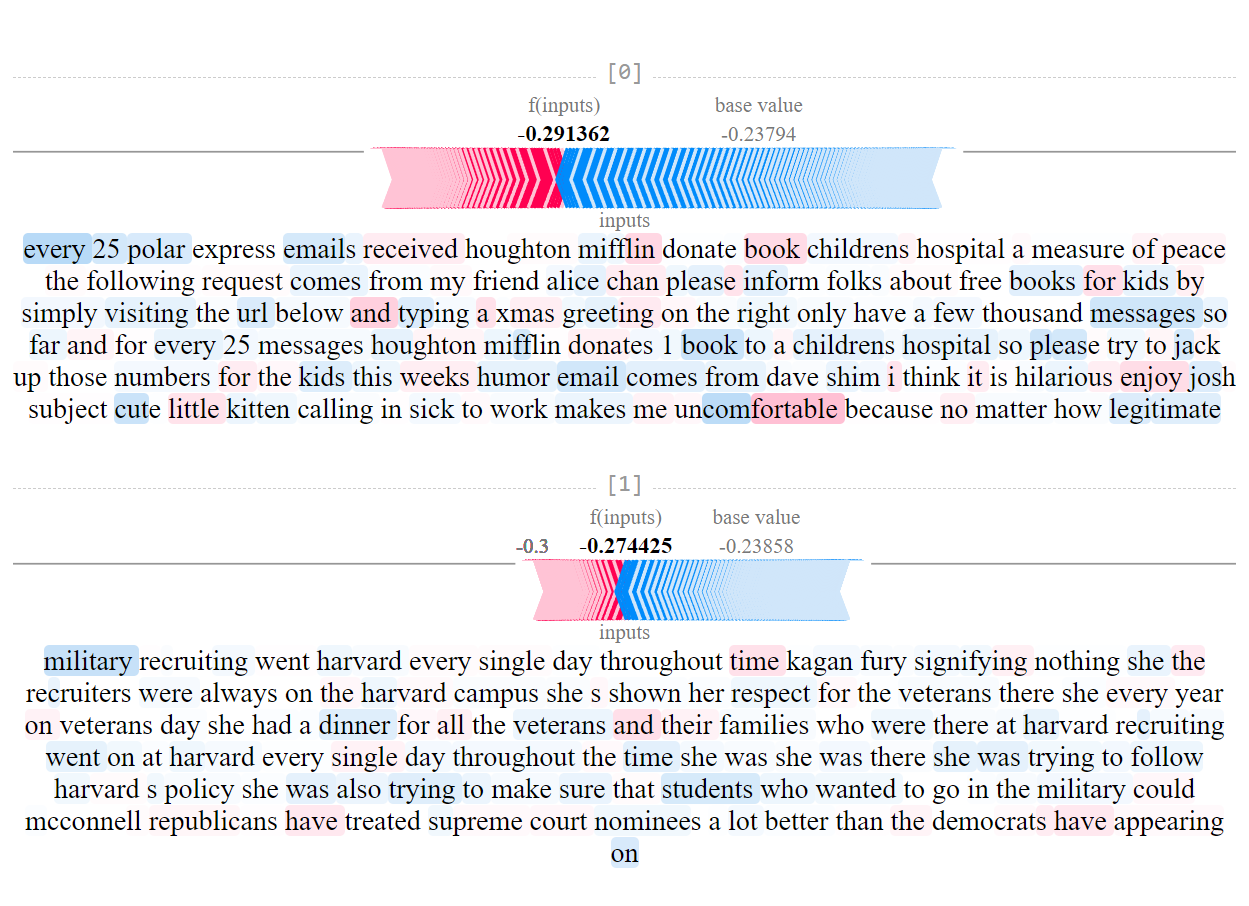
\includegraphics[width=\textwidth]{figs/one-distil-b-ml-c.png}
        % \caption{{DistilBERT}\textsubscript{B, C}}
    \endminipage\hfill % maximize horizontal separation
    \minipage{0.32\textwidth}
        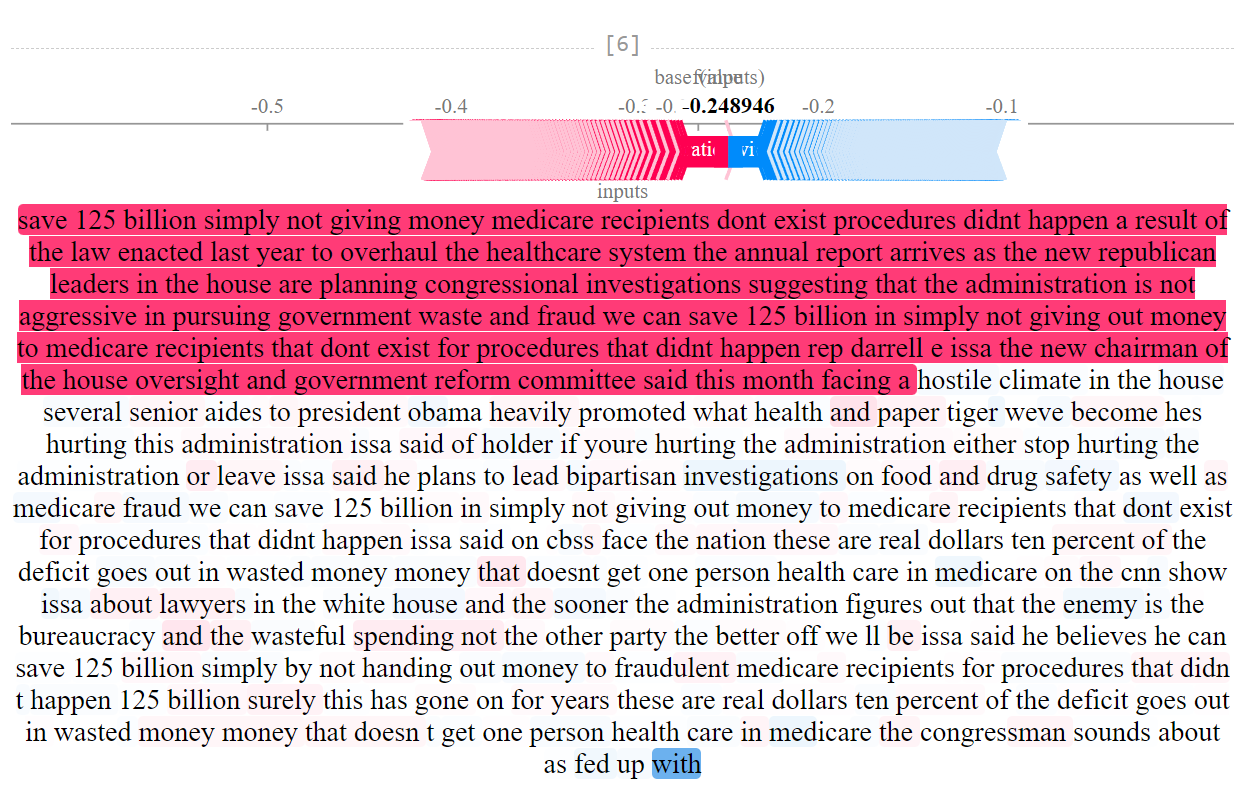
\includegraphics[width=\textwidth]{figs/all-distil-b-ml-c.png}
        % \caption{{DistilBERT}\textsubscript{B, C}}
    \endminipage\hfill % maximize horizontal separation
    \minipage{0.32\textwidth}
        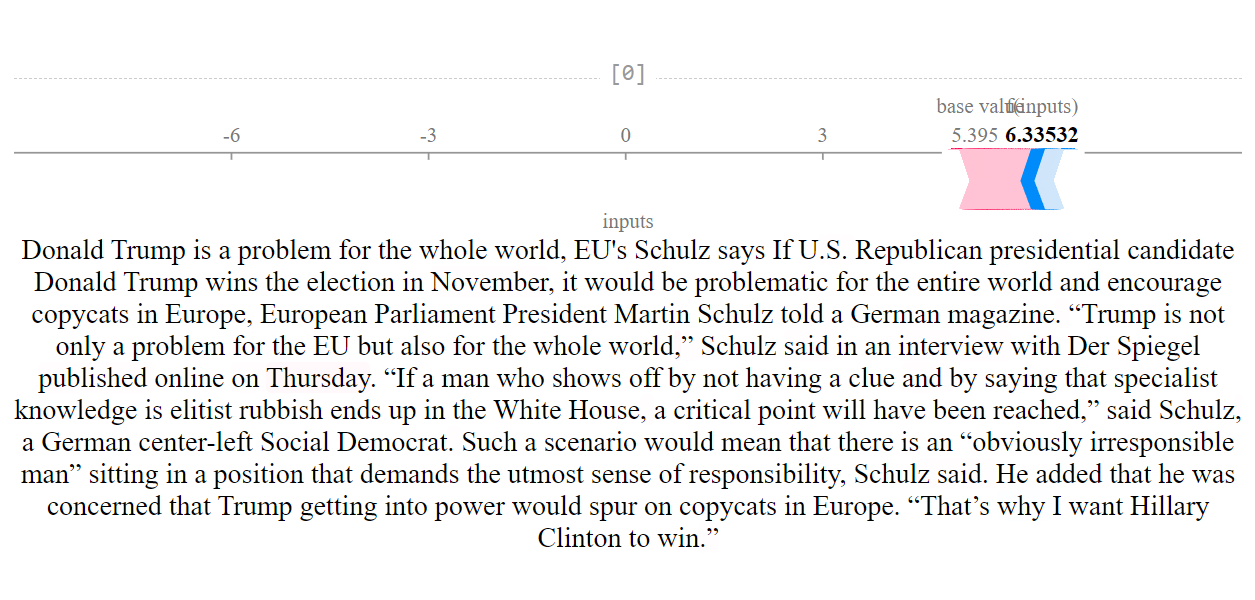
\includegraphics[width=\linewidth]{figs/news-distil-b-ml-c.png}
        % \caption{{DistilBERT}\textsubscript{B, C, ML}}
    \endminipage
    
    \caption{Valores Shapley de {DistilBERT}\textsubscript{B, C, ML} para los tres \textit{datasets}.}
    % \label{fig:shap-ps-one}
\end{figure}

\begin{itemize}
    \item LARGE, CASED, ML \textit{vs.} otros\footnote{Existen algunas excepciones según \textit{dataset} y modelo}.
    \item Rendimiento general: {P-S}\textsubscript{All} $>$ {P-S}\textsubscript{One} $>$ {News}.
\end{itemize}

\end{frame}

\begin{frame}{5.7. Evaluación}
\begin{itemize}
    \item LARGE ofrece resultados más consistentes.
    \item Alto valor de \textit{specificity}: gran capacidad de detectar noticias verdaderas.
    \item Análisis cuantitativo \textit{vs.} cualitativo: resultados generalmente poco concluyentes; distinto a lo esperado (\textit{datasets}, modelos...).
\end{itemize}
    
\end{frame}